\documentclass[11pt]{article}

\usepackage[margin=1in]{geometry}
\usepackage[T1]{fontenc}
\usepackage[utf8]{inputenc}
\usepackage{mathpazo}
\usepackage{microtype}
\usepackage{setspace}
\usepackage{enumitem}
\usepackage{titlesec}
\usepackage{xcolor}
\usepackage{hyperref}
\usepackage{tikz}
\usepackage{caption}

\usetikzlibrary{arrows.meta, positioning, shapes.geometric, fit}

\definecolor{fiBlue}{HTML}{1F4E79}
\definecolor{fiSlate}{HTML}{566475}
\definecolor{fiRule}{HTML}{D6DCE2}
\definecolor{fiBox}{HTML}{F7F9FB}
\definecolor{fiBoxBorder}{HTML}{A8B7C5}

\hypersetup{
  colorlinks=true,
  linkcolor=fiBlue,
  urlcolor=fiBlue,
  pdftitle={Future Invest: Toward an AI-Native Investment Institution},
  pdfauthor={Codex},
  pdfsubject={Academic text version with workflow figure}
}

\setstretch{1.08}
\setlength{\parindent}{0pt}
\setlength{\parskip}{0.58em}
\setlist[itemize]{leftmargin=1.5em, itemsep=0.25em, topsep=0.3em}
\setlist[enumerate]{leftmargin=1.5em, itemsep=0.25em, topsep=0.3em}

\titleformat{\section}{\large\bfseries\color{black}}{\thesection.}{0.6em}{}
\titleformat{\subsection}{\normalsize\bfseries\color{fiBlue}}{\thesubsection}{0.6em}{}

\begin{document}

\begin{center}
{\small\textsc{\textcolor{fiBlue}{Text Edition}}}\par
\vspace{0.5em}
{\LARGE\bfseries Future Invest: Toward an AI-Native Investment Institution for Long/Short Equity Research, Execution Design, and Capital Allocation\par}
\vspace{0.75em}
{\normalsize Academic reading version prepared from the repository proposal source\par}
\vspace{0.35em}
{\small \textcolor{fiSlate}{Source file: \texttt{docs/future-invest-proposal.md}}}
\end{center}

\vspace{0.8em}
\hrule
\vspace{1em}

\begin{abstract}
This proposal introduces \textbf{Future Invest}, an AI-native investment institution designed for long/short equity research, execution design, and portfolio-aware capital allocation. The central argument is that current multi-agent finance systems remain too close to human organizational charts: they are interpretable, but they are often static, weakly capital-aware, and effectively stateless across runs. Future Invest addresses this gap by combining four design elements within a unified operating system: capability-native research modules, institution-level orchestration, front-loaded portfolio constraints, and durable institutional memory. Instead of asking isolated agents to produce disconnected reports, the system coordinates a shared dossier that integrates business truth, market expectations, timing, catalysts, execution planning, and capital allocation logic. The proposal advances the hypothesis that such a system will generate more coherent, more portfolio-aware, and more testable investment decisions than both static role-based multi-agent baselines and simplified single-agent baselines. The repository already contains a working runtime, a batch evaluation harness, and persistent memory infrastructure, allowing the proposal to be evaluated not only as a conceptual design but also as an empirical systems contribution.
\end{abstract}

\section{Motivation}

Modern investment organizations face a persistent bottleneck: high-quality investment cognition is fragmented across functions, expensive to scale, and slow to recombine. Fundamental long/short platforms are often strongest at company understanding, industry structure, financial modeling, and long-horizon variant perception. However, they may be weaker in short-cycle timing, catalyst compression, and portfolio-level execution speed. By contrast, multi-manager and faster long/short equity platforms often excel in portfolio discipline, timing, and rapid capital allocation, but they can underinvest in durable company understanding and long-horizon mispricing.

An AI-native institution should not merely imitate one of these legacy structures, nor should it simply translate a human org chart into software. The more ambitious opportunity is to combine deep business understanding with faster timing, explicit portfolio constraints, and institutional learning. Future Invest is motivated by that opportunity.

\section{Problem Statement}

Most current multi-agent systems in finance still decompose work into fixed human-like roles such as analyst, trader, risk manager, and portfolio manager. This is useful for interpretability, but it leaves several structural limitations unresolved:

\begin{itemize}
\item workflows are usually fixed rather than dynamically routed;
\item capital allocation is often treated as a terminal stage rather than a standing constraint;
\item long-cycle mispricing, medium-cycle re-rating, and short-cycle execution are frequently conflated;
\item memory is shallow, so systems repeatedly reason from scratch instead of compounding institutional knowledge;
\item evaluation is often anecdotal, with limited infrastructure for comparing system variants over historical cases.
\end{itemize}

The result is that many systems are better at generating research-style narratives than at behaving like a genuine investment institution.

\section{Research Objective}

The objective of this project is to design and evaluate an AI-native investment institution that combines:

\begin{itemize}
\item the depth of fundamental long/short investing,
\item the timing and portfolio discipline of faster platform-style investing,
\item and the compounding advantage of machine memory and adaptive workflow control.
\end{itemize}

The practical goal is not simply to produce better reports. It is to build a system that can generate decisions that are clearer, more falsifiable, more portfolio-aware, and easier to evaluate over time.

\section{Proposed System}

Future Invest is designed around four architectural principles.

\subsection{Capability-Native Research}

The front-end research layer is organized around investment questions rather than legacy job titles:

\begin{itemize}
\item \textbf{Business Truth}: What is economically real about the company?
\item \textbf{Market Expectations}: What is already priced into the market?
\item \textbf{Timing \& Catalysts}: Why does the idea matter on this horizon, what event chain could force a re-rating, and what signals would invalidate that timing?
\end{itemize}

This decomposition is intended to reduce role mimicry and sharpen the informational function of each module.

\subsection{Institution-Level Orchestration}

An \textbf{Investment Orchestrator} acts as the institutional control layer rather than a static scheduler. It determines:

\begin{itemize}
\item which capability modules to activate,
\item whether additional research is worth the token and time budget,
\item when to intensify counterevidence search,
\item when to stop research and move into execution and capital formation.
\end{itemize}

In other words, the orchestrator allocates research effort in response to uncertainty, evidence conflict, and mandate importance.

\subsection{Capital-Aware Decision Protocol}

Portfolio reasoning is surfaced early instead of being appended after thesis formation. Before the thesis is finalized, the system constructs:

\begin{itemize}
\item a \textbf{Portfolio Mandate},
\item a \textbf{Time Horizon Split},
\item an \textbf{Institutional Memory Brief}.
\end{itemize}

This makes the downstream workflow explicitly conditional on portfolio role, risk budget, capital budget, and temporal structure.

\subsection{Long-Term Institutional Memory}

Future Invest maintains durable company-level memory that includes:

\begin{itemize}
\item world model history,
\item thesis history,
\item prediction ledger,
\item agent reliability memory.
\end{itemize}

This memory is meant to let the system behave more like a persistent institution and less like a stateless assistant.

\section{Workflow Overview}

Figure~\ref{fig:workflow} summarizes the proposed workflow in a text-friendly academic format.

\begin{figure}[htbp]
\centering
\resizebox{\linewidth}{!}{%
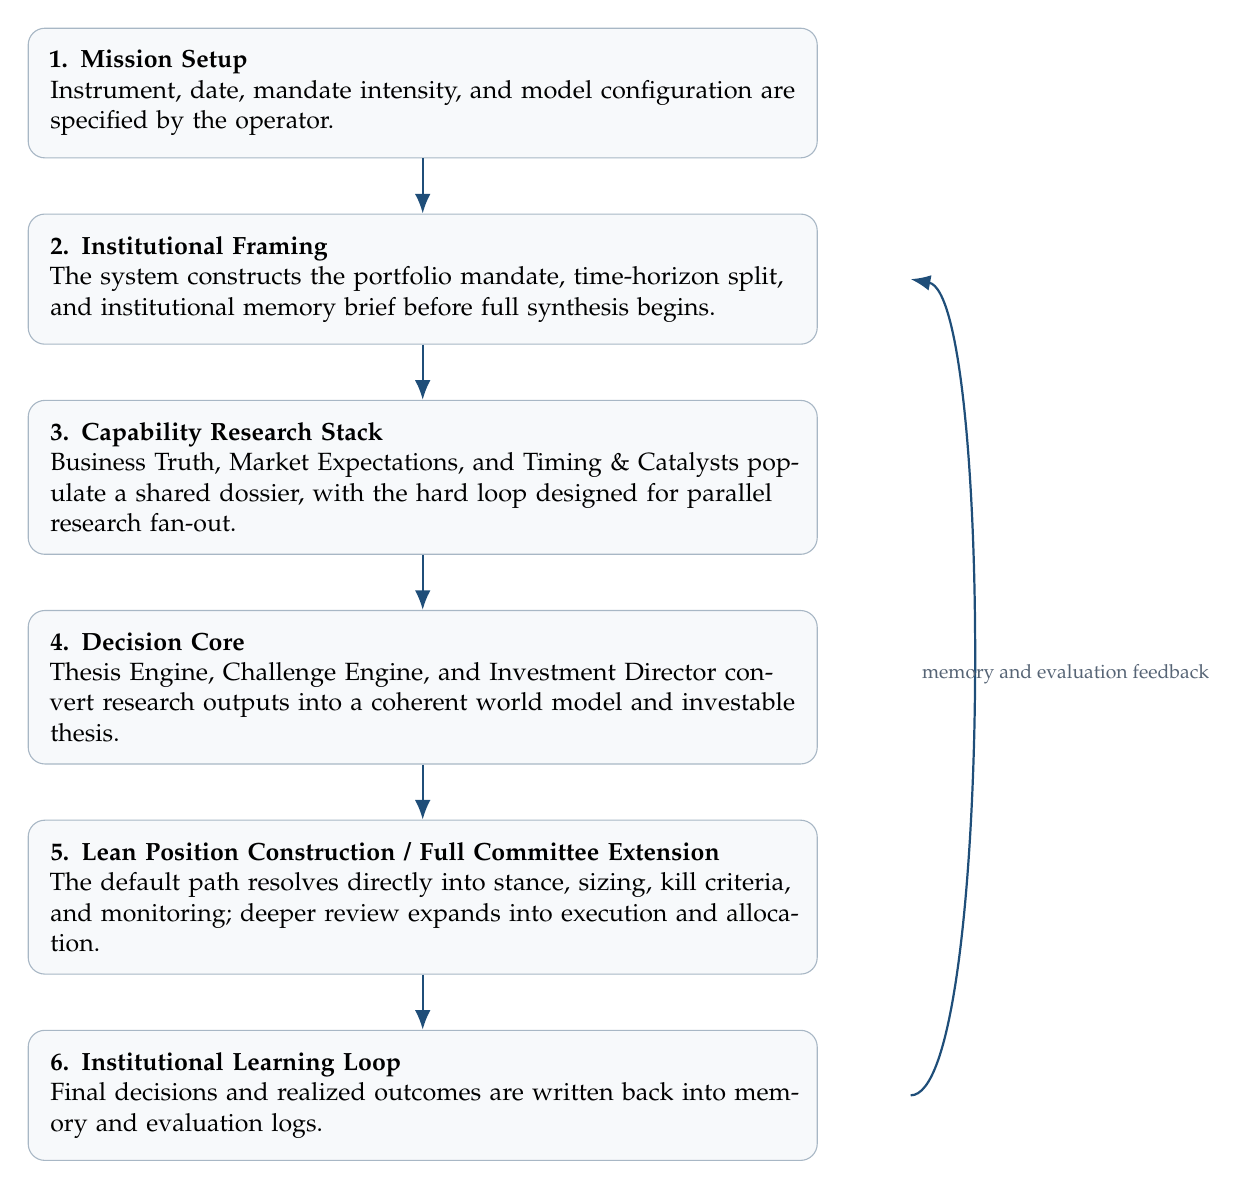
\begin{tikzpicture}[
  node distance=7mm and 10mm,
  stage/.style={
    draw=fiBoxBorder,
    rounded corners=6pt,
    fill=fiBox,
    text width=0.78\linewidth,
    minimum height=1.15cm,
    align=left,
    inner sep=8pt,
    font=\small
  },
  arrow/.style={-{Latex[length=2.5mm,width=2mm]}, thick, draw=fiBlue}
]

\node[stage] (s1) {\textbf{1. Mission Setup}\\Instrument, date, mandate intensity, and model configuration are specified by the operator.};
\node[stage, below=of s1] (s2) {\textbf{2. Institutional Framing}\\The system constructs the portfolio mandate, time-horizon split, and institutional memory brief before full synthesis begins.};
\node[stage, below=of s2] (s3) {\textbf{3. Capability Research Stack}\\Business Truth, Market Expectations, and Timing \& Catalysts populate a shared dossier, with the hard loop designed for parallel research fan-out.};
\node[stage, below=of s3] (s4) {\textbf{4. Decision Core}\\Thesis Engine, Challenge Engine, and Investment Director convert research outputs into a coherent world model and investable thesis.};
\node[stage, below=of s4] (s5) {\textbf{5. Lean Position Construction / Full Committee Extension}\\The default path resolves directly into stance, sizing, kill criteria, and monitoring; deeper review expands into execution and allocation.};
\node[stage, below=of s5] (s6) {\textbf{6. Institutional Learning Loop}\\Final decisions and realized outcomes are written back into memory and evaluation logs.};

\draw[arrow] (s1.south) -- (s2.north);
\draw[arrow] (s2.south) -- (s3.north);
\draw[arrow] (s3.south) -- (s4.north);
\draw[arrow] (s4.south) -- (s5.north);
\draw[arrow] (s5.south) -- (s6.north);
\draw[arrow] ([xshift=1.18cm]s6.east) .. controls +(1.05,0) and +(1.05,-0.2) .. ([xshift=1.18cm]s2.east);
\node[anchor=west, text=fiSlate, font=\scriptsize] at ([xshift=1.2cm,yshift=0.16cm]s4.east) {memory and evaluation feedback};
\end{tikzpicture}
}
\caption{Future Invest begins with mission setup and institutional framing, routes through a capability-native research stack, synthesizes outputs through a decision core, resolves through a lean position-construction loop by default, optionally expands into a fuller committee path, and finally writes outcomes back into institutional memory and evaluation logs.}
\label{fig:workflow}
\end{figure}

At a high level, the workflow proceeds in six stages:

\begin{enumerate}
\item \textbf{Mission Setup}. The operator specifies the instrument, date, mandate intensity, and model configuration.
\item \textbf{Institutional Framing}. The orchestrator constructs the initial portfolio mandate, time-horizon split, and institutional memory brief.
\item \textbf{Capability Research Stack}. Business Truth, Market Expectations, and Timing \& Catalysts populate a shared dossier, with the research layer designed to run in parallel inside the hard loop.
\item \textbf{Decision Core}. Thesis Engine, Challenge Engine, and Investment Director convert research outputs into a coherent world model and investable thesis.
\item \textbf{Lean Position Construction / Full Committee Extension}. The default lean loop resolves directly into stance, sizing, kill criteria, and monitoring. When deeper review is required, the system expands into execution and allocation engines.
\item \textbf{Institutional Learning Loop}. Final decisions and realized outcomes are recorded into persistent memory and evaluation logs.
\end{enumerate}

\section{Research Questions and Hypotheses}

The proposal is organized around one primary question:

\begin{quote}
Can an AI-native investment institution produce more coherent, more capital-aware, and more evaluable investment decisions than role-based or single-agent baselines?
\end{quote}

This question is decomposed into four hypotheses.

\subsection*{H1. Research Quality}
Capability-native decomposition will improve thesis clarity, counterevidence quality, and world-model coherence relative to role-based baselines.

\subsection*{H2. Temporal Discipline}
Explicit separation of long-cycle mispricing, medium-cycle re-rating, and short-cycle execution will improve the distinction between ``good company'' and ``good trade right now.''

\subsection*{H3. Portfolio Discipline}
Front-loaded portfolio constraints will improve portfolio-role clarity, sizing discipline, kill criteria, and trade-to-book fit.

\subsection*{H4. Institutional Learning}
Persistent institutional memory will improve cross-run consistency and reduce repeated analytical failure over time.

\section{Evaluation Design}

The repository already contains a batch evaluation harness in \href{file:///Users/x/Desktop/my_aider_code/codex/TradingAgents/evaluation/run_eval.py}{\texttt{evaluation/run\_eval.py}}. This makes the proposal empirically testable inside the codebase itself.

Evaluation should proceed on four layers.

\subsection{Engineering Reliability}
\begin{itemize}
\item run success rate,
\item latency and runtime dispersion,
\item structural completeness of canonical sections,
\item robustness to case variation and configuration changes.
\end{itemize}

\subsection{Research Quality}
\begin{itemize}
\item thesis clarity,
\item counterevidence strength,
\item portfolio mandate clarity,
\item time-horizon separation,
\item dossier completeness.
\end{itemize}

\subsection{Institution Quality}
\begin{itemize}
\item usefulness of execution planning,
\item explicitness of kill criteria,
\item capital-budget discipline,
\item portfolio-fit reasoning,
\item consistency across repeated runs.
\end{itemize}

\subsection{Outcome Quality}
\begin{itemize}
\item distribution of final ratings,
\item forward return buckets,
\item hit rate,
\item realized drawdown,
\item post-hoc error analysis by module, regime, and decision stage.
\end{itemize}

The most informative experimental design is a structured comparison across at least three systems:

\begin{itemize}
\item the original role-based multi-agent workflow,
\item the current Future Invest workflow,
\item a simplified single-agent baseline.
\end{itemize}

\section{Expected Contribution}

This project is expected to contribute in three ways.

\subsection{Systems Contribution}
It offers a concrete architecture for AI-native investing that replaces static role replication with adaptive orchestration, explicit portfolio context, temporal decomposition, and durable memory.

\subsection{Methodological Contribution}
It proposes a way to evaluate investment agents as institutions rather than only as single-run forecasters. This includes engineering metrics, research-quality metrics, institution-quality metrics, and outcome metrics.

\subsection{Conceptual Contribution}
It reframes the role of AI in investing. The core claim is not that one more agent or one better prompt solves the problem, but that the unit of design should be the institution itself.

\section{Scope and Limitations}

This project does not claim to solve the entire problem of real-world asset management. Several limitations remain important:

\begin{itemize}
\item outputs remain sensitive to model quality, prompt design, and data vendor coverage;
\item the current portfolio layer is still more textual than fully state-driven;
\item realized investment performance depends on execution assumptions and market regime;
\item system improvement must be demonstrated through repeated evaluation rather than asserted from isolated examples.
\end{itemize}

These limitations are not peripheral; they define the next frontier of work.

\section{Why This Matters}

If successful, Future Invest provides a blueprint for a new category of investment organization: one that combines the depth of fundamental long/short research, the speed and discipline of modern platform investing, and the compounding advantage of machine memory and workflow optimization.

The broader ambition is therefore not to build a better report generator. It is to prototype the operating system of a future investment institution.

\vspace{1em}
\hrule
\vspace{0.6em}

{\small\textcolor{fiSlate}{This academic-style PDF was prepared as a text-first reading version. The workflow figure was redrawn to preserve a clean manuscript presentation.}}

\end{document}
